\documentclass{article}
\usepackage[margin=1.25in]{geometry}
\usepackage{amsmath, amssymb, setspace, enumerate, enumitem}
\usepackage{setspace}
\usepackage{graphicx}
\onehalfspacing

\begin{document}
    \begin{enumerate}
        \item Exercise 3.4
        \begin{enumerate}[label=(\alph*)]
            \item we know $y = w^{*T}x + \epsilon$ and $H = X(X^TX)^-1X^T$ from (3.6), and we know $\hat{y} = Hy$ by definition, we want to prove $\hat{y} = Xw^* + H\epsilon$
            \begin{align*}
                \hat{y} &= H(w^*X + \epsilon)\\
                &= X(X^TX)^{-1}X^T(w^*X+\epsilon)\\
                &= X(X^TX)^{-1}X^Tw^*X + X(X^TX)^{-1}X^T\epsilon\\
                &= w^*X + H\epsilon
            \end{align*}

            \item for $\hat{y} - y$, we have
            \begin{align*}
                \hat{y} - y &= w^*X + H\epsilon - (w^* + \epsilon)\\
                &= H\epsilon - \epsilon\\
                &= \epsilon(H - I)
            \end{align*}
            where $I$ denotes the identity matrix

            \item let $E_{in}(w) = \frac{1}{N} ||\hat{y} - y||^2$
            \begin{align*}
                E_{in}(w) &= \frac{1}{N}||\epsilon(H-I)||^2\\
                &= \frac{1}{N}(\epsilon(H - I))^T(\epsilon(H - I))\\
                &= \frac{1}{N}\epsilon^T(H-I)^T\epsilon(H-I)\\
            \end{align*}
            We know $H - I$ is symmetric, so $(H-I)^T = (H-I)$
            \begin{align*}
                E_{in}(w) &= \frac{1}{N}\epsilon^T\epsilon(H-I)^2\\
                &= \frac{1}{N}\epsilon^T\epsilon(I - H)^2
            \end{align*}

            \item We know
            \begin{align*}
                E_D[E_{in}(w_{lin})] &= E_D[\frac{1}{N}(\epsilon^T\epsilon(I - H))]\\
                &= \frac{1}{N} (E_D[\epsilon^T\epsilon] - E_D[\epsilon^T\epsilon H])\\
            \end{align*}
            Given that $\epsilon$ is a noise term with zero mean and $\sigma^2$ variance. The variance of each noise component $\epsilon$ is $\sigma^2$, so 
            \begin{align*}
                E_D[E_{in}(w_{lin})] &= \frac{1}{N}(N\sigma^2 - E_D[\epsilon^T\epsilon H])\\
                &= \sigma^2 - \frac{1}{N}E_D[\epsilon^T\epsilon H]
            \end{align*}
            
            Now we can calculate
            \begin{align*}
                E_D[\epsilon^T\epsilon H] &= E_D[\sum_{i = 1}^{N}\epsilon_i^2 H]\\
                &= H \sum_{i = 1}^{N}E_D[\epsilon_i^2]
            \end{align*}

            By the problem, we know that each component of $\epsilon$ is a random variable with zero mean and variance $\sigma^2$, so this means that $E_D[\epsilon_i] = 0$ and $E_D[\epsilon_i^2] = \sigma^2$ for all $i$.
            \begin{align*}
                E_D[\epsilon^T\epsilon H] &= H\sum_{i = 1}^{N} \sigma^2\\
                &= HN\sigma^2
            \end{align*}

            We continue the problem by substituting the result into our original equation
            \begin{align*}
                E_D[E_{in}(w_{lin})] = \sigma^2 - \frac{1}{N} E_D[\epsilon^T\epsilon H] &= \sigma^2 - \frac{1}{N}HN\sigma^2\\
                &= \sigma^2 - H\sigma^2
            \end{align*}

            Then, we can calculate for the $trace(H)$
            \begin{align*}
                trace(H) &= trace(X(X^T X)^{-1} X^T)\\
                &= trace((X^TX)^{-1}(X^TX))
            \end{align*}

            Given that $X^T X$ is a square matrix of size $(d + 1)$, and it's inverse $(X^TX)^{-1}$ is also present, then we have
            \begin{align*}
                trace((X^TX)^{-1}(X^TX)) &= d + 1\\
                trace(H) &= \frac{d + 1}{N}
            \end{align*}

            Then, we have proved that $E_D[E_{in}(w_{lin})] = \sigma^2 ( 1 - \frac{d + 1}{N}) \hfill\blacksquare$
            
            \item to do
            \begin{align*}
                E_{D, \epsilon^\prime}[E_{test}(w_{lin})] = E_{D, \epsilon^\prime}[\frac{1}{N}||Xw - y^\prime||^2]
            \end{align*}
            
        \end{enumerate}

        \item Problem 3.1
        \begin{enumerate}[label=(\alph*)]
            \item 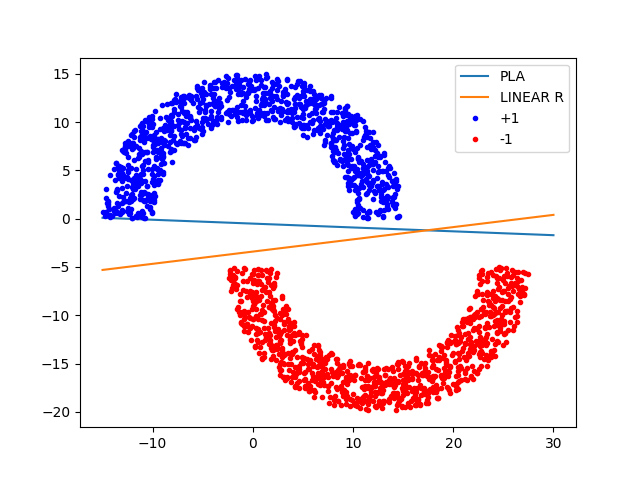
\includegraphics[scale=0.5]{images/p3_1.png}
            \item Both PLA and linear regression found ways to separate this data, however, one could say that the linear regression algorithm found a better way to separate the data as the PLA appears to be closer to the top part of the semicircle, barely missing on misclassifying one of the $+1$ points. With this, one can predict that linear regression will have a lower $E_{out}$ than the PLA, however, this isn't guaranteed.
        \end{enumerate}
    \end{enumerate}
\end{document}